\documentclass{article}

\usepackage{amsmath}
\usepackage{amssymb}
\usepackage{enumerate}
\usepackage[spanish]{babel}
\usepackage{cancel}
\usepackage{caption}
\usepackage[margin=1.5in]{geometry}
\usepackage{graphicx}
\usepackage[utf8]{inputenc}
\usepackage{tcolorbox}
\usepackage{esint}
\usepackage{hyperref}
\hypersetup{
    colorlinks,
    citecolor=black,
    filecolor=black,
    linkcolor=black,
    urlcolor=black,
}

\renewcommand{\Bbb}{\mathbb}

\tcbuselibrary{theorems}

\title{Ejercicios de Análisis Matemático II A (63.01) \\
Guía 3 - Diferenciabilidad, tangentes \\
Cátedra Acero \\
1° C 2004}
\author{Darío Eduardo Ramos}

\begin{document}
\maketitle

\tableofcontents{}
\newpage

\section*{3.1}
\label{sec:3.1}
\addcontentsline{toc}{section}{\nameref{sec:3.1}}

\textbf{En los siguientes casos:} 

\begin{enumerate}
\bfseries

\item Calcular el gradiente de $f$ en el punto $P_0 = (x_0, y_0)$
\item En un gráfico en 3D, trazar aproximadamente la curva de nivel $C$ de $f$ que pasa por $P_0$, su recta tangente en $P_0$ y el gradiente de $f$ con origen en $P_0$.
\item (En el mismo gráfico) Ubicar el punto $Q_0$ de la superficie $z = f(x,y)$ cuya proyección en el plano $xy$ es $P_0$; dibujar aproximadamente la superficie $z$ en la vecindad de $Q_0$ y su plano tangente.
\item (En el mismo gráfico) Marcar sobre la superficie $z$ la curva cuya proyección en el plano $xy$ es $C$.
\item (En el mismo gráfico) Graficar el vector $N = (f'_x(P_0), f'_y(P_0), -1)$ con origen en $Q_0$.
\item ¿Qué relación hay entre los distintos objetos geométricos del gráfico? Explicar las relaciones con palabras y ponerlas en evidencia en los dibujos.

\end{enumerate}

\begin{enumerate}[(a)]
\bfseries

\item $f(x,y)=x^2+y^2, P_0 = (1,1)$
\item $f(x,y)=\sqrt{4-x^2-y^2}, P_0 = (1,-1)$
\item $f(x,y)=5+2x-3y, P_0=(0,0)$
\item $f(x,y)=7+xy, P_0=(0,0)$
\item $f(x,y)=7+x^2-y^2, P_0=(1,1)$
\item $f(x,y)=\sqrt{x^2+y^2/4}, P_0=(0,2)$

\end{enumerate}
\hrule

\subsection*{3.1.a}
\label{subsec:3.1.a}
\addcontentsline{toc}{subsection}{\nameref{subsec:3.1.a}}

\subsubsection*{3.1.a.1}
\label{subsubsec:3.1.a.1}
\addcontentsline{toc}{subsubsection}{\nameref{subsubsec:3.1.a.1}}

Por simple inspección, $f \in C^1$ y por ende existe el gradiente:

\begin{equation}
\overrightarrow{ \nabla f }(x,y) = (f_x(x,y), f_y(x,y)) = (2x, 2y)
\end{equation}

Ergo:

\begin{equation}
\tcboxmath[colback=orange!25!white,colframe=orange,title=3.1.a.1]
{
\overrightarrow{ \nabla f }(x_0,y_0) = (2, 2)
}
\end{equation}

\subsubsection*{3.1.a.2}
\label{subsubsec:3.1.a.2}
\addcontentsline{toc}{subsubsection}{\nameref{subsubsec:3.1.a.2}}

La curva de nivel $k$ de f es:

\begin{equation}
C_k(f) = \{ (x,y) \in \Bbb R^2 / x^2 + y^2 = k, k \in \Bbb R, k \geq 0 \}
\end{equation}

Por lo tanto, la curva de nivel asociada a $P_0$ es:

\begin{equation}
(x_0)^2 + (y_0)^2 = 2 \Rightarrow k = 2
\end{equation}

\begin{equation}
\tcboxmath[colback=orange!25!white,colframe=orange,title=3.1.a.2]
{
C_2(f) = \{ (x,y) \in \Bbb R^2 / x^2 + y^2 = 2 \}
}
\end{equation}

Para hallar la recta tangente a $C_2(f)$, conviene parametrizarla como curva en $\Bbb R^2$. Es un círculo de radio $\sqrt{2}$, por ende:

\begin{subequations}
\begin{align}
& C_2(f): \sigma(t) = (\sqrt{2} \cos(t), \sqrt{2} \sin(t)), t \in [0, 2\pi) \\
& \sigma'(t) = (-\sqrt{2} \sin(t), \sqrt{2} \cos(t))
\end{align}
\end{subequations}

Ahora bien, el punto donde se desea evaluar la recta tangente es $(x_0, y_0) = (1, 1)$. Sea $t_0$ el valor que hace $\sigma(t_0) = (x_0, y_0)$. El próximo paso es calcular ese valor.

\begin{equation}
(\sqrt{2} \cos(t_0), \sqrt{2} \sin(t_0)) = (1, 1) \Rightarrow t_0 = \frac{\pi}{4}
\end{equation}

El vector dirección de la recta tangente en $\sigma(t_0)$ es $\sigma'(t_0) = (-1, 1)$. La recta tangente en $(1, 1)$ es entonces:

\begin{equation}
\tcboxmath[colback=orange!25!white,colframe=orange,title=3.1.a.2]
{
L_T: (-1, 1) \alpha + (1, 1)
}
\end{equation}

Gráficamente, estos elementos pueden visualizarse en la figura \ref{fig:1-a-2}.

\begin{figure}[ht]
\caption{Curva de nivel, recta tangente y gradiente}
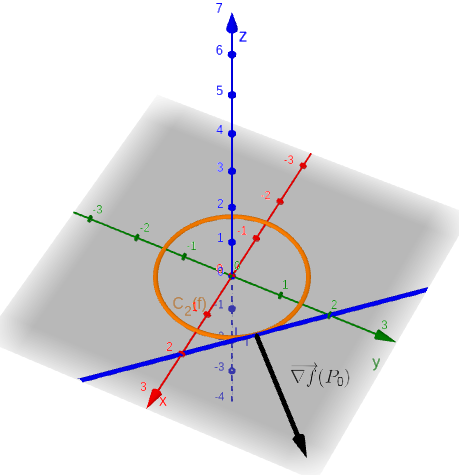
\includegraphics[scale=0.35]{img/ejercicios/3/1-a-2.png} 
\centering
\label{fig:1-a-2}
\end{figure}

Nótese que el gradiente, tomando como origen el vector $(x_0, y_0)$, es un vector ortogonal al vector dirección de la recta tangente.

\subsubsection*{3.1.a.3}
\label{subsubsec:3.1.a.3}
\addcontentsline{toc}{subsubsection}{\nameref{subsubsec:3.1.a.3}}

Primero, para calcular el plano tangente en un punto $P_0$, recúerdese que ello puede realizarse usando las derivadas parciales:

\begin{equation}
\Pi_T: z-z_0 - f_x(P_0) (x-x_0) - f_y(P_0) (y-y_0) = 0
\end{equation}

Para este caso, $x_0 = 1$, $y_0 = 1$, $z_0 = 2$, $f_x(x,y) = 2x$, y $f_y(x,y) = 2y$. Ergo:

\begin{subequations}
\begin{align}
& z-2 - 2 (x-1) - 2(y-1) = 0 \\
& z-2 -2x +2 -2y +2 = 0 \\
& -2x -2y + z + 2 = 0
\end{align}
\end{subequations}

\begin{equation}
\tcboxmath[colback=orange!25!white,colframe=orange,title=3.1.a.3]
{
\Pi_T: 2x + 2y -z -2 = 0
}
\end{equation}

La superficie asociada a $z = x^2 + y^2$ es un paraboloide centrado en el origen. El punto $Q_0$ no es otra cosa que $(x_0, y_0, f(x_0, y_0)) = (1, 1, 2)$. Agregando la superficie y el plano tangente al gráfico previo, se obtiene la figura \ref{fig:1-a-3}.

\begin{figure}[ht]
\caption{Superficie y plano tangente}
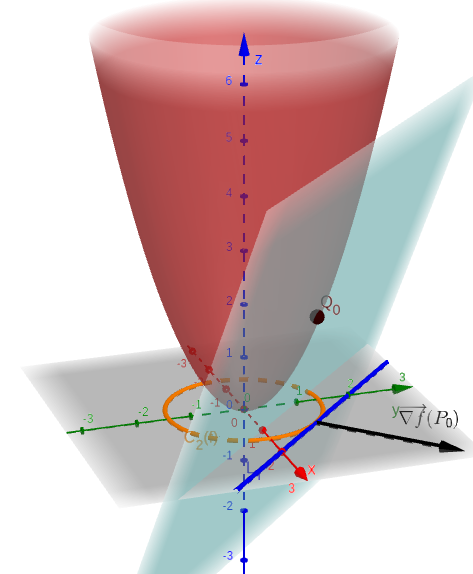
\includegraphics[scale=0.35]{img/ejercicios/3/1-a-3.png} 
\centering
\label{fig:1-a-3}
\end{figure}

\end{document}
